\begin{figure}[ht]
    % ROW 1
    \begin{subfigure}[t]{.25\textwidth}
        \begin{subfigure}[t]{\textwidth}
            \caption{}
            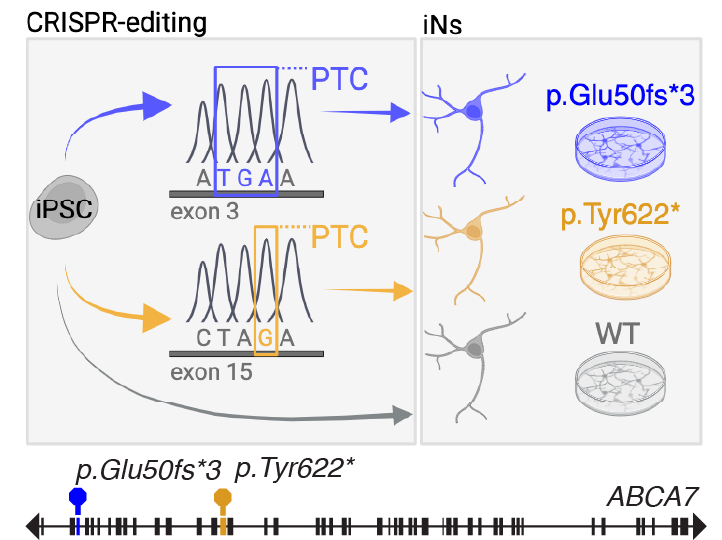
\includegraphics[width=\textwidth]{./main_plots/iN_cartoon.png}        
        \end{subfigure} 
        \begin{subfigure}[t]{\textwidth}
            \caption{}
            \includegraphics[width=\textwidth]{./extended_plots/rna_correlation_both_lof_lines.png}        
        \end{subfigure} 
    \end{subfigure} 
    \begin{subfigure}[t]{.25\textwidth}
        \begin{subfigure}[t]{\textwidth}
            \caption{}
            \includegraphics[width=\textwidth]{./main_plots/y622_kl_clusters_network.pdf}        
        \end{subfigure}
        \begin{subfigure}[t]{\textwidth}
            \caption{}
            \centering
            \includegraphics[width=0.5\textwidth]{./main_plots/jaccard_cartoon.png}        
            \includegraphics[width=\textwidth]{./extended_plots/jaccard_PM_pT622.png}        
        \end{subfigure}  
    \end{subfigure} 
    \begin{subfigure}[t]{.5\textwidth}
        \caption{}
        \includegraphics[width=\textwidth]{./main_plots/kl_densities_Tyr622.png}        
    \end{subfigure}  
    % Row 2
    \begin{subfigure}[t]{.3\textwidth}
        \begin{subfigure}[t]{\textwidth}
            \caption{}
            \includegraphics[width=\textwidth]{./main_plots/y622_mito_degs.png}        
        \end{subfigure}  
    \end{subfigure} 
    \begin{subfigure}[t]{.2\textwidth}
        \caption{}
            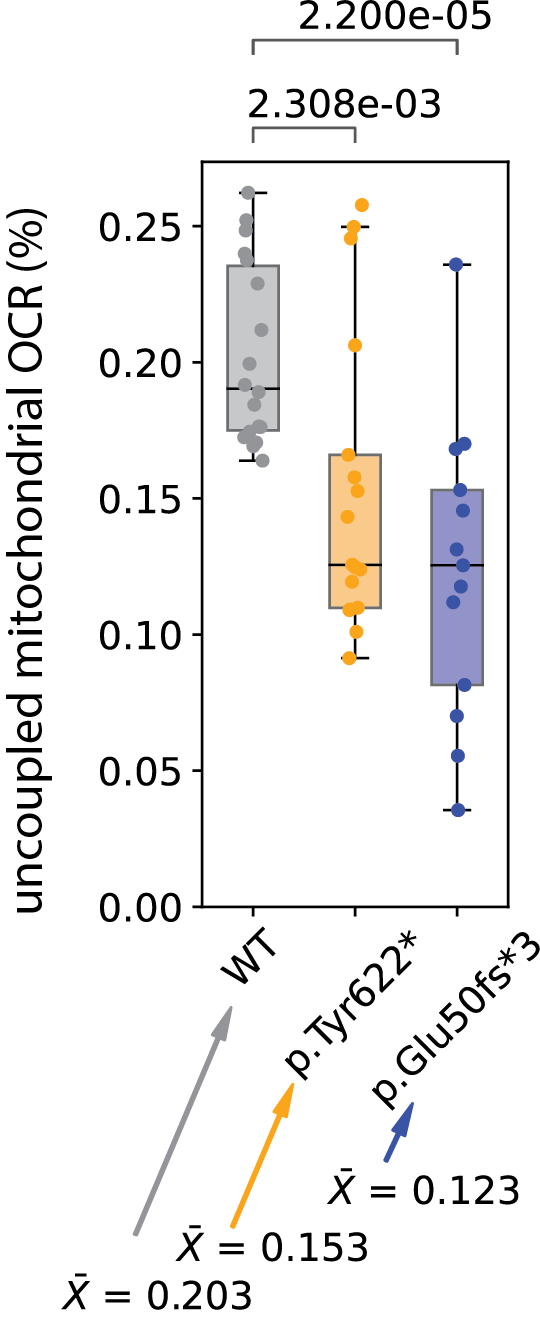
\includegraphics[width=\textwidth]{./main_plots/uncoupling.png}        
    \end{subfigure}   
    \begin{subfigure}[t]{.5\textwidth}
        \caption{}
        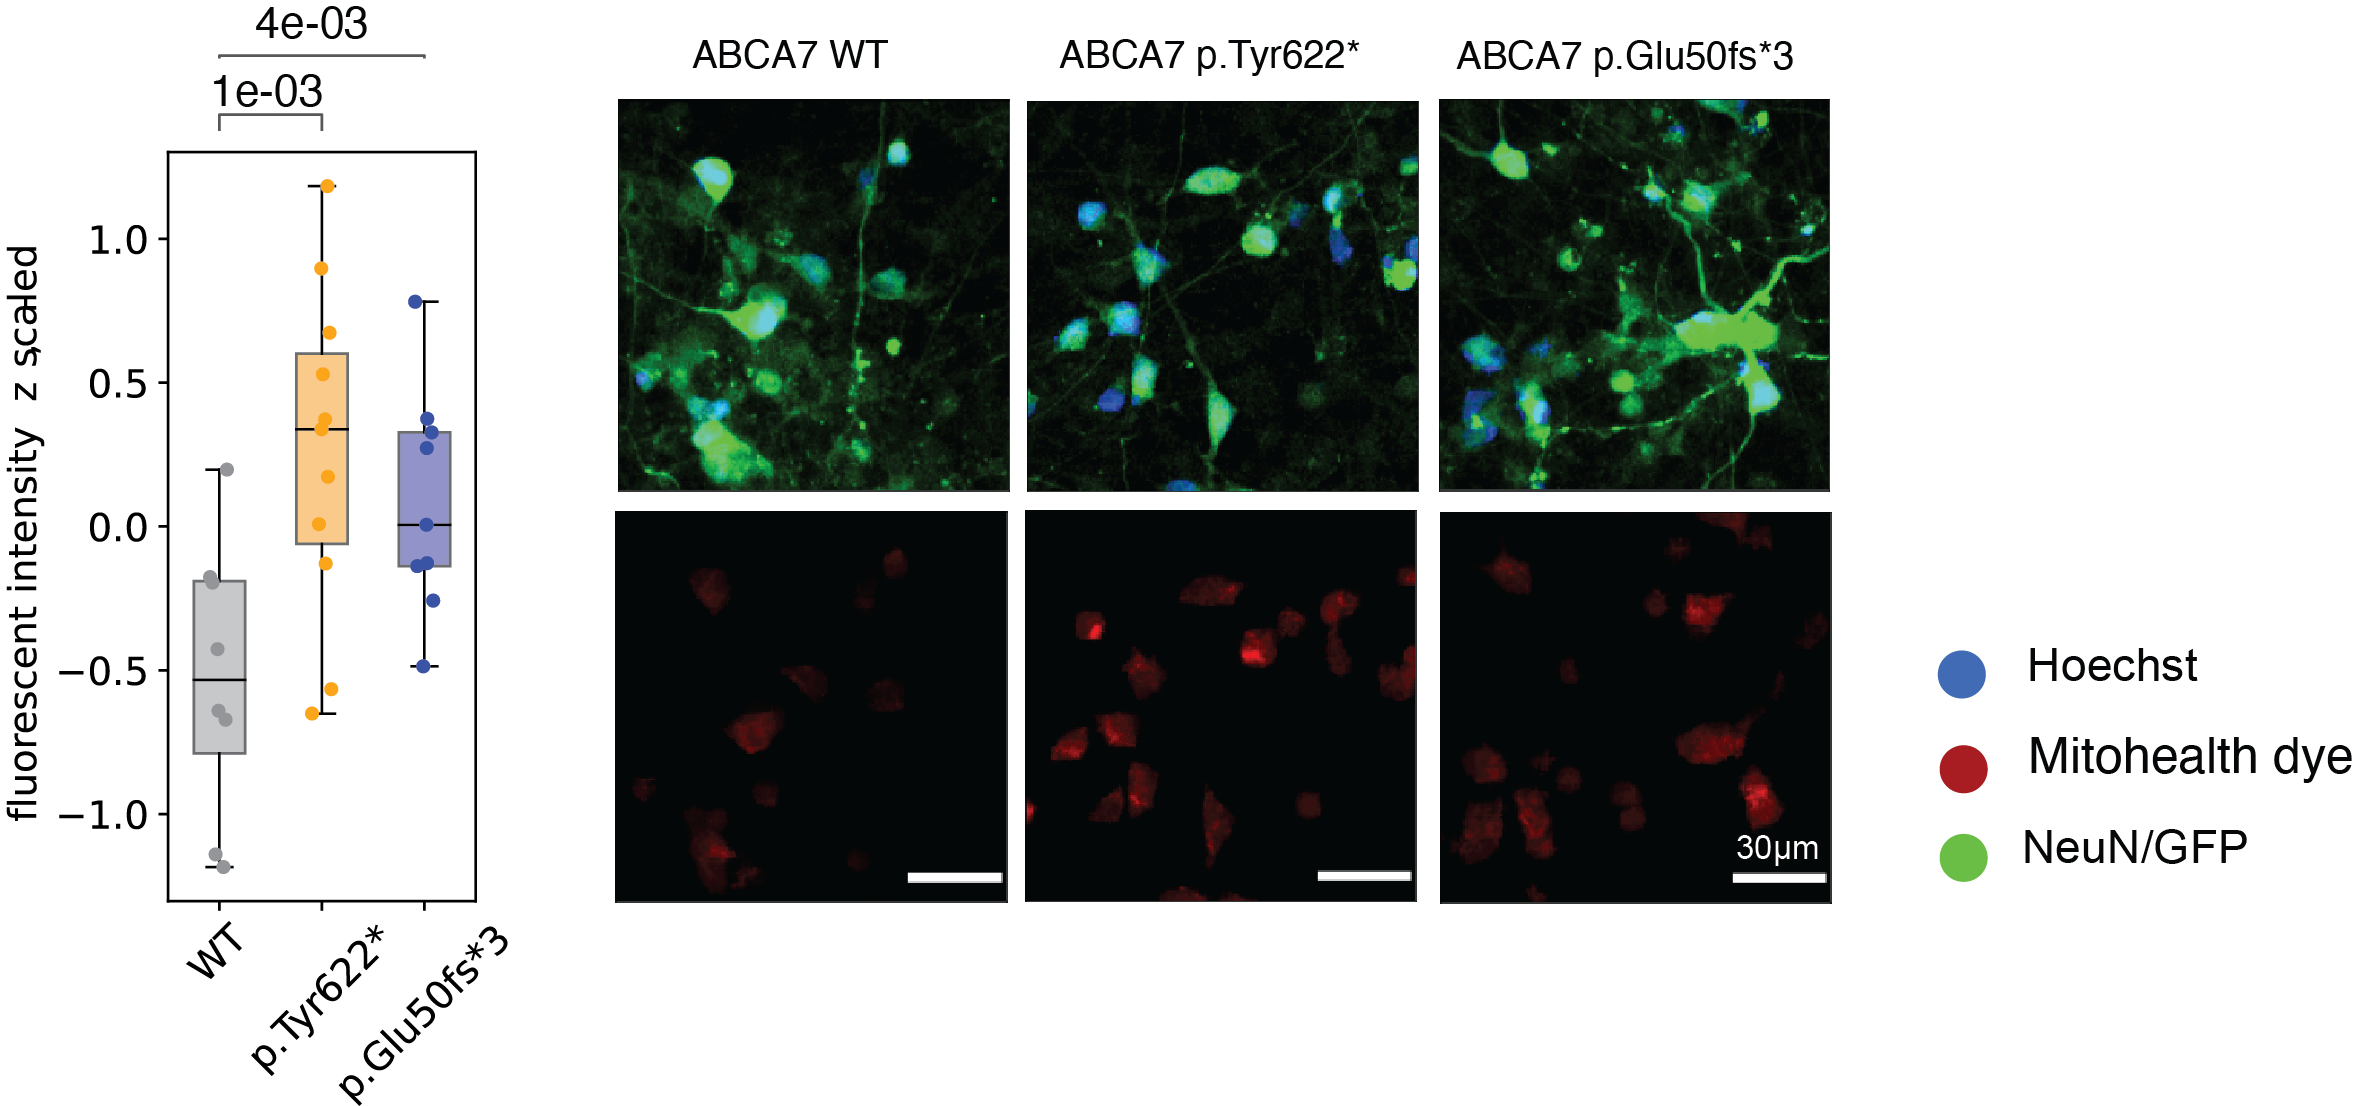
\includegraphics[width=\textwidth]{./extended_plots/mitohealth_dye.png}        
    \end{subfigure}    
    % Row 3
    \begin{subfigure}[t]{.4\textwidth}
        \caption{}
        \includegraphics[width=\textwidth]{./main_plots/tmrm_with_FCCP.png}        
    \end{subfigure}    
   % \hspace{1cm}
    \begin{subfigure}[t]{.3\textwidth}
        \caption{}
        \includegraphics[width=\textwidth]{./main_plots/cellrox_images.png}        
    \end{subfigure}  
    \begin{subfigure}[t]{.3\textwidth}
        \caption{}
        \includegraphics[width=\textwidth]{./main_plots/all_lipids_y622.png}        
    \end{subfigure}  


    % \begin{subfigure}[t]{.2\textwidth}
    %     \begin{subfigure}[t]{\textwidth}
    %         \caption{}
    %         \includegraphics[width=\textwidth]{./extended_plots/jaccard_pT622_pG50fs3_vs_wt.png}        
    %     \end{subfigure} 
    %     \begin{subfigure}[t]{\textwidth}
    %         \caption{}
    %         \includegraphics[width=\textwidth]{./main_plots/jaccard_PM_pT622.png}        
    %     \end{subfigure} 
    % \end{subfigure} 
    % \begin{subfigure}[t]{.3\textwidth}
    %     \caption{}
    %     \includegraphics[width=\textwidth]{./main_plots/jaccard_pT622_pG50fs3_vs_wt.png}        
    % \end{subfigure}  
    % \begin{subfigure}[t]{.45\textwidth}
    %     \caption{}
    %     \includegraphics[width=\textwidth]{./main_plots/kl_densities_Tyr622.png}        
    % \end{subfigure}   
    % % ROW 2 & 3

    % % ROW 2

    %     \begin{subfigure}[t]{.6\textwidth}
    %         \caption{}
    %         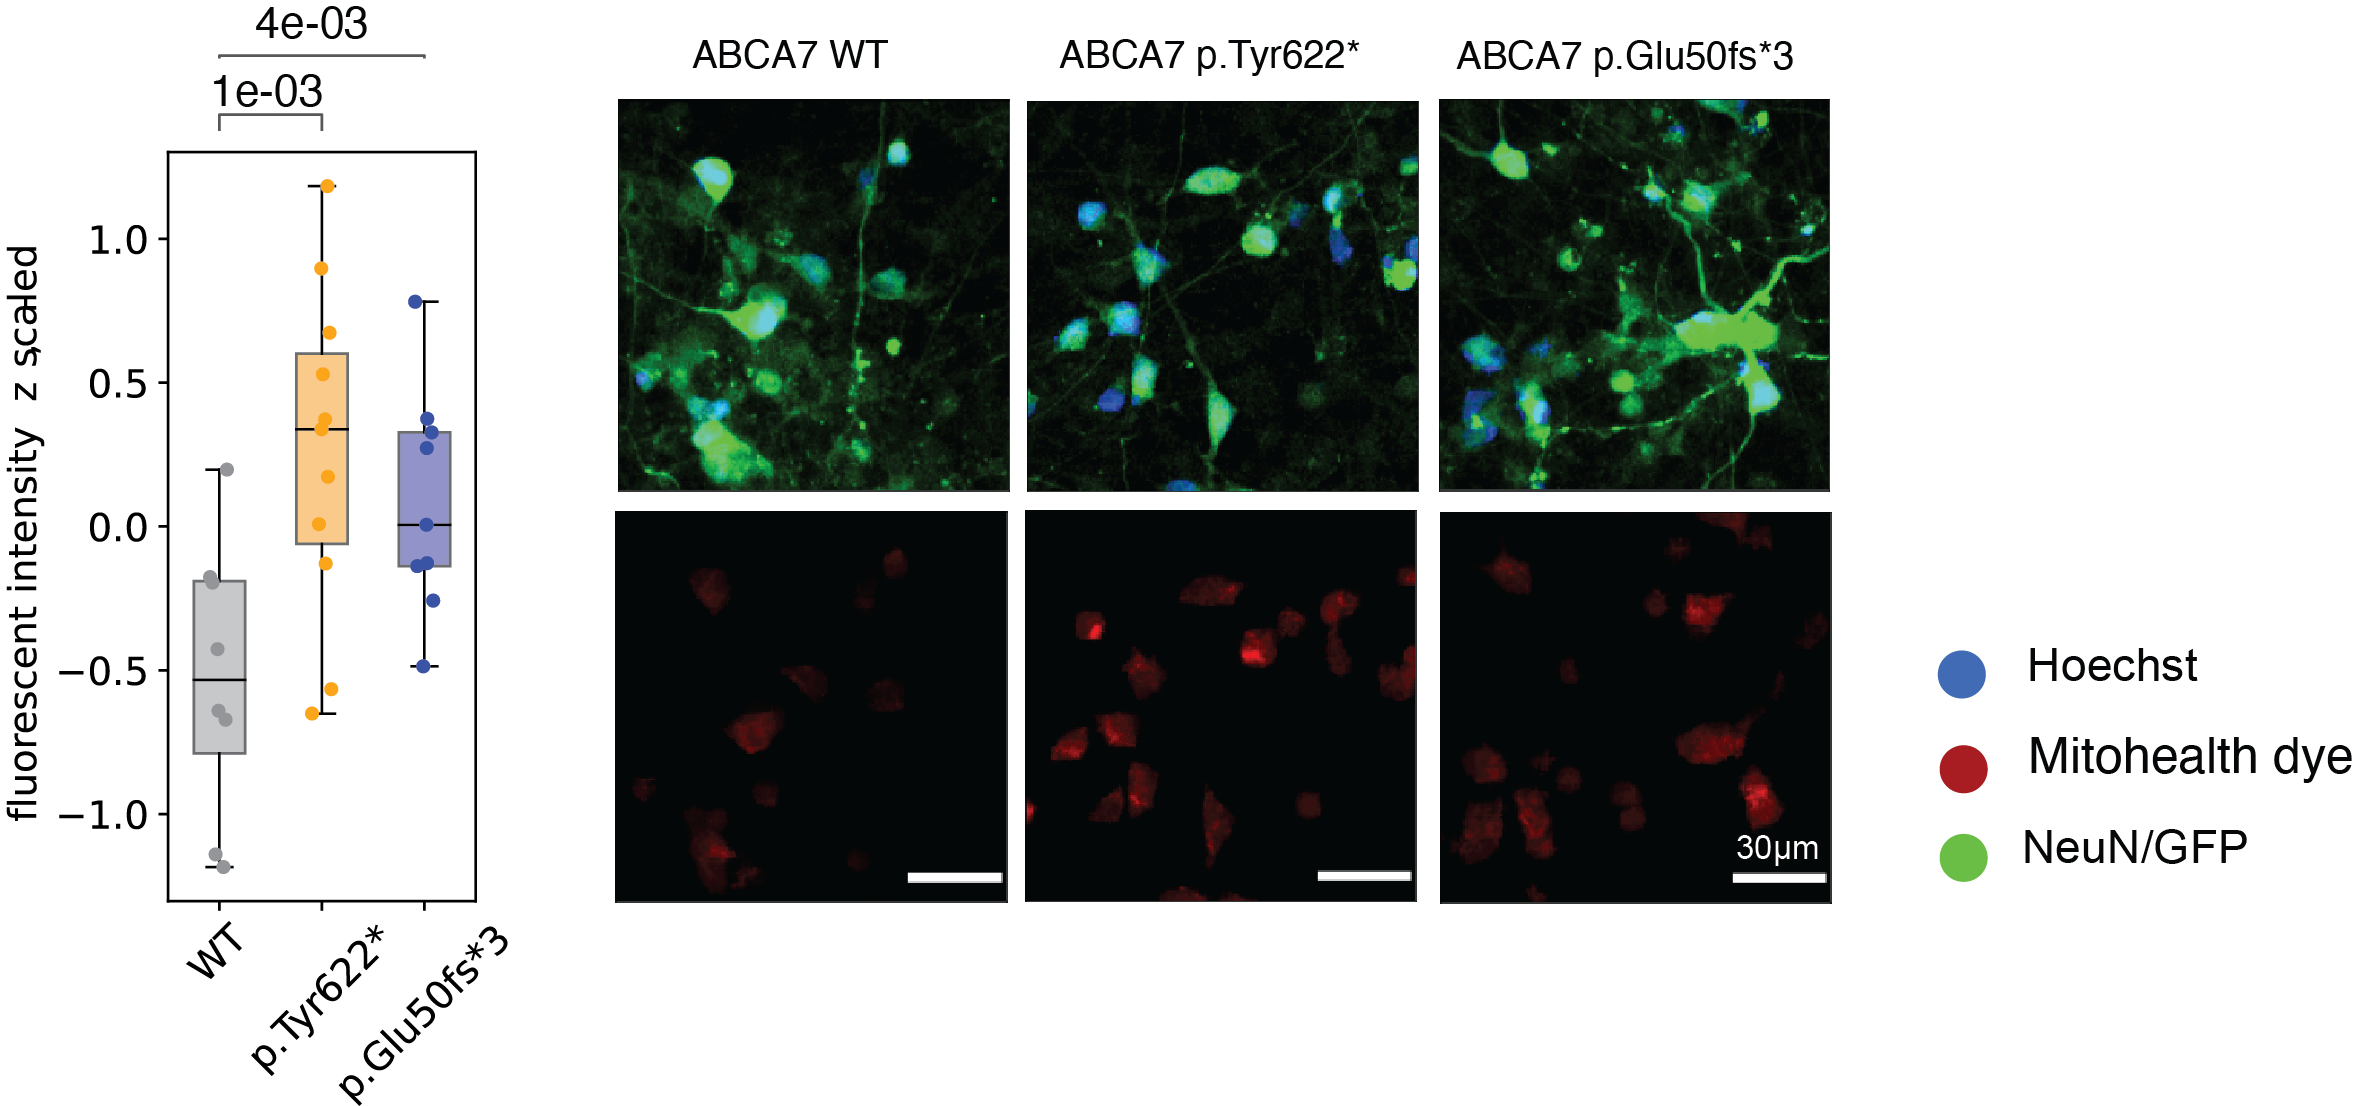
\includegraphics[width=\textwidth]{./extended_plots/mitohealth_dye.png}        
    %     \end{subfigure}     
    %     \par
    %     \begin{subfigure}[t]{.65\textwidth}
    %         \caption{}
    %         \includegraphics[width=\textwidth]{./main_plots/tmrm_with_FCCP.png}        
    %     \end{subfigure}     
    %     \begin{subfigure}[t]{.35\textwidth}
    %         \caption{}
    %         \includegraphics[width=\textwidth]{./main_plots/y622_mito_degs.png}        
    %     \end{subfigure}    
    % \end{subfigure}     
    %\includegraphics[width=\textwidth]{./main_plots/fig_4_temp.png}  
    % \begin{subfigure}[t]{.5\textwidth}
    %     \begin{subfigure}[t]{.3\textwidth}
    %         \begin{subfigure}[t]{\textwidth}
    %             \caption{}
    %             \includegraphics[width=\textwidth]{./main_plots/E3_vs_Y622_kl_network.pdf}        
    %         \end{subfigure} 
    %         \begin{subfigure}[t]{\textwidth}
    %             \caption{}
    %             \includegraphics[width=\textwidth]{./extended_plots/e3_y622_jaccard.png}        
    %         \end{subfigure} 
    %     \end{subfigure}
    %     \begin{subfigure}[t]{.7\textwidth}
    %         \caption{}
    %         \includegraphics[width=\textwidth]{./main_plots/e3_y622_density.pdf}        
    %     \end{subfigure}  
    % \end{subfigure}
    % \begin{subfigure}[t]{.3\textwidth}
    %     \caption{}
    %     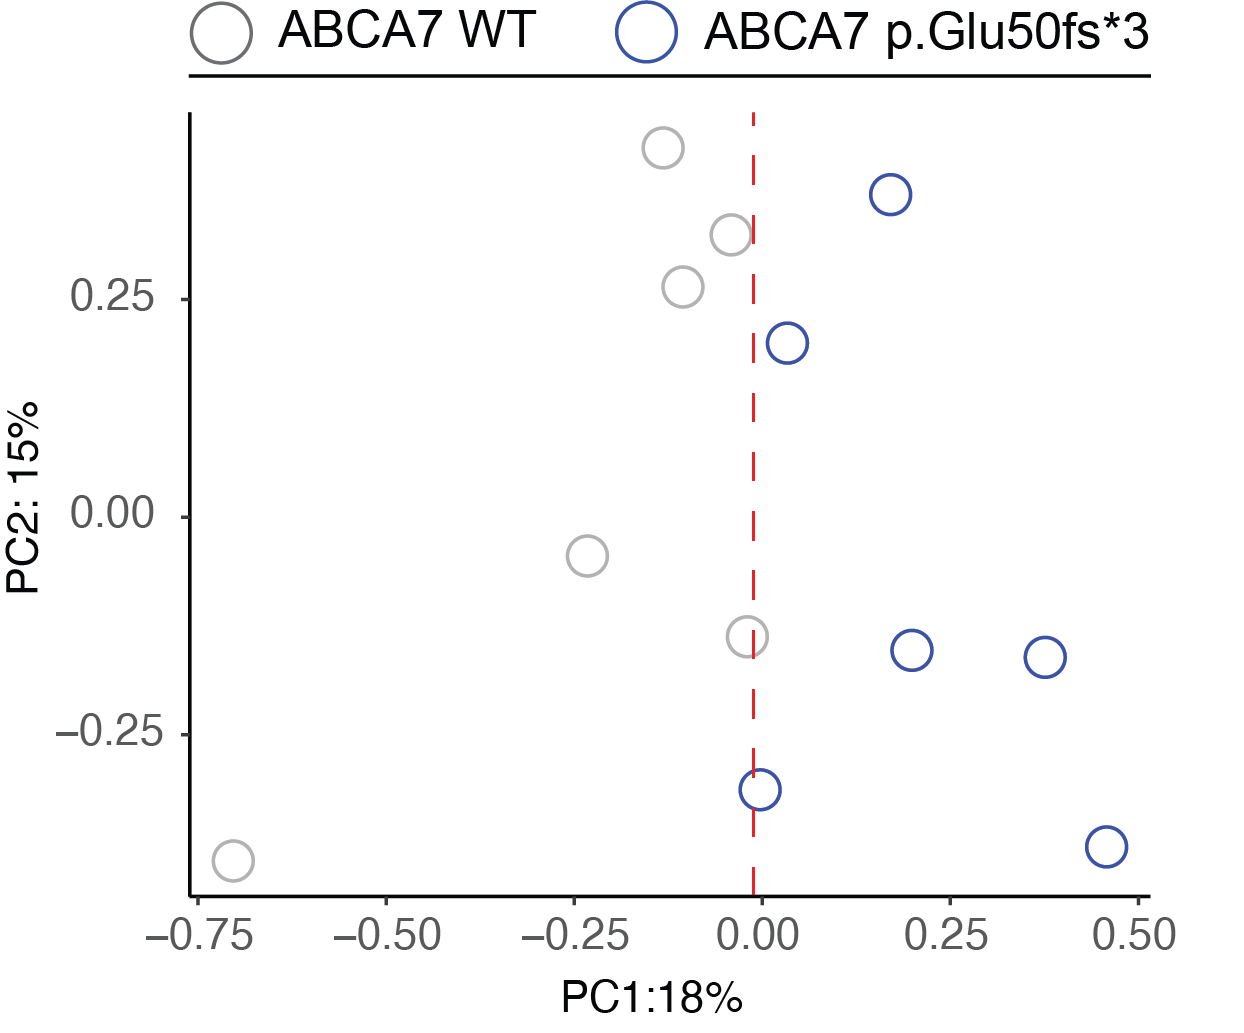
\includegraphics[width=\textwidth]{./main_plots/metabolomics_pca.png}        
    % \end{subfigure}   
    % \begin{subfigure}[t]{.3\textwidth}
    %     \caption{}
    %     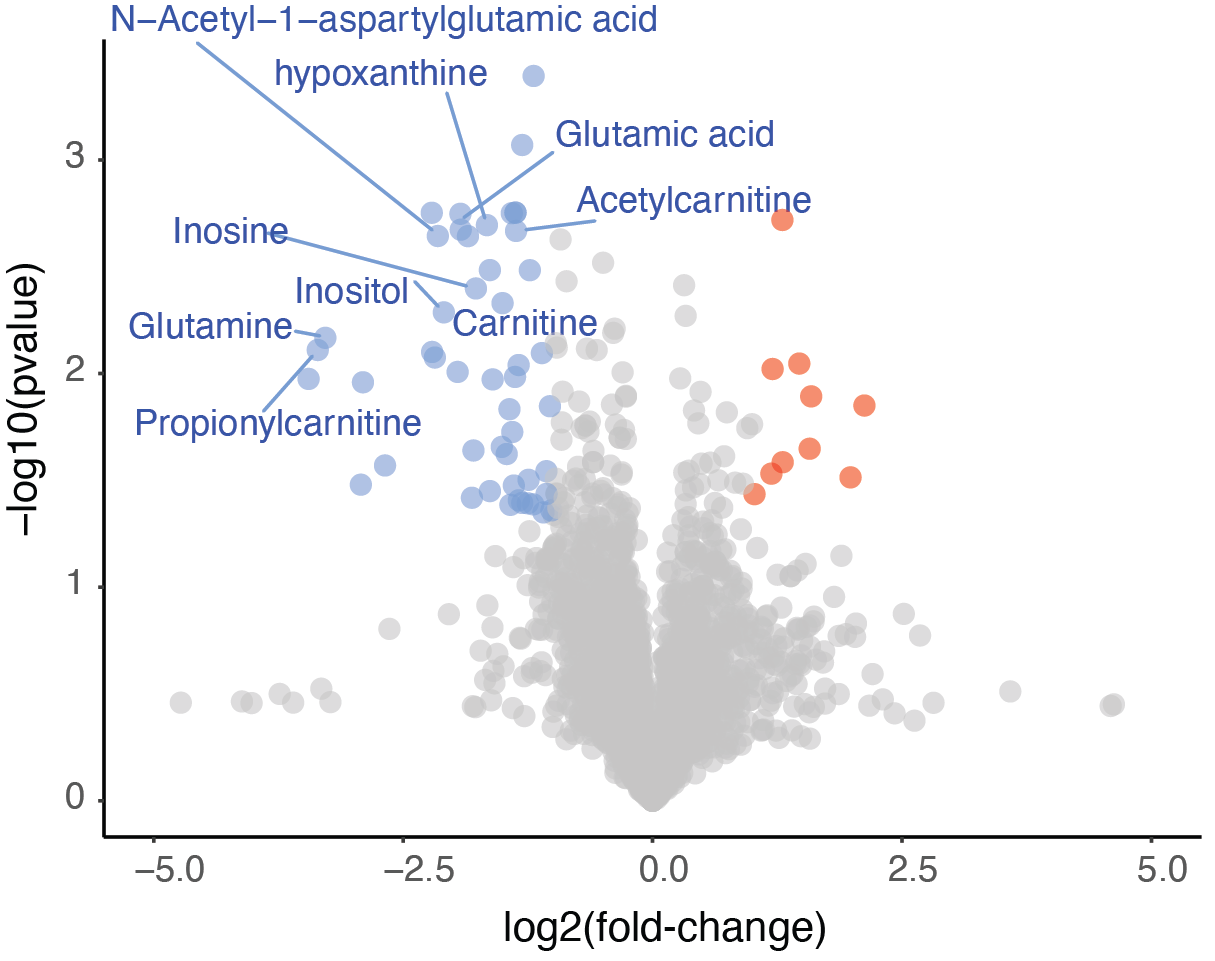
\includegraphics[width=\textwidth]{./main_plots/metabolomics_volcano.png}        
    % \end{subfigure}   
    % \begin{subfigure}[t]{.4\textwidth}
    %     \caption{}
    %     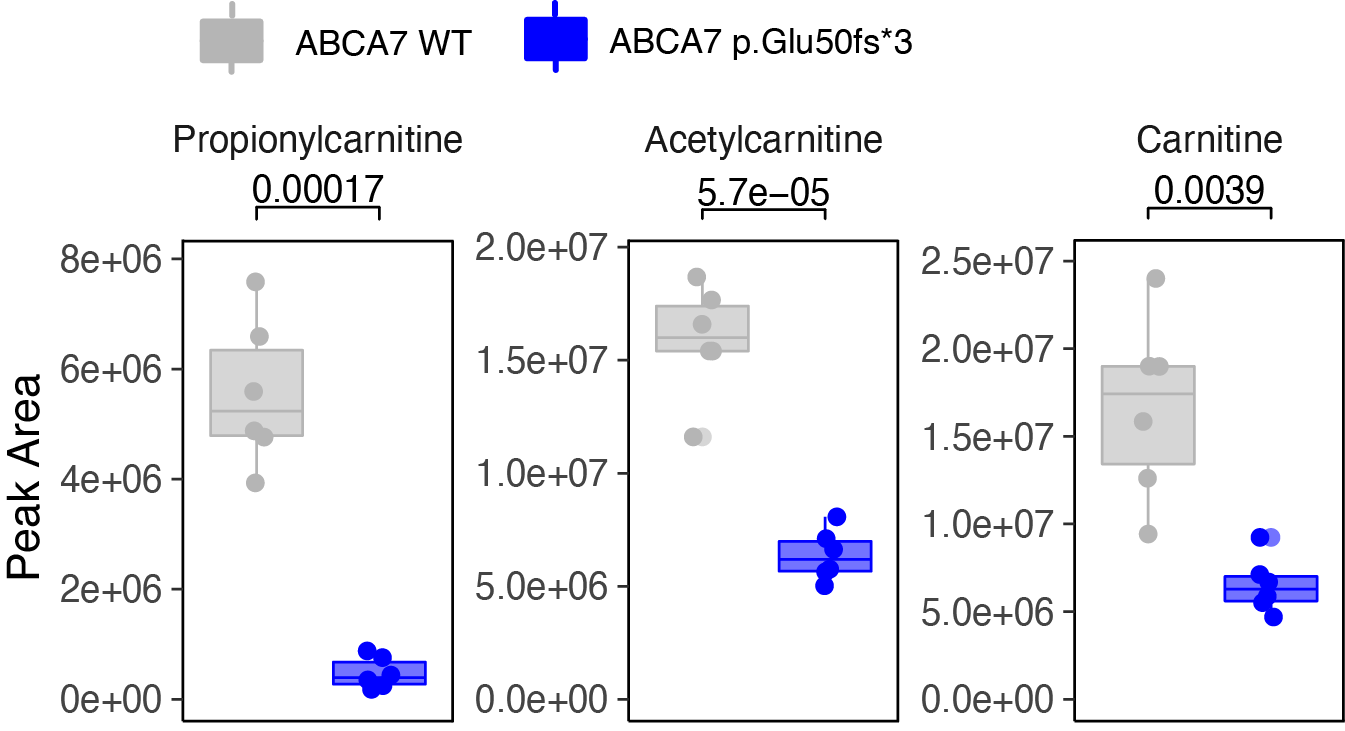
\includegraphics[width=\textwidth]{./main_plots/metab_species.png}        
    % \end{subfigure}   
    % \begin{subfigure}[t]{.3\textwidth}
    %     \begin{subfigure}[t]{0.9\textwidth}
    %         \caption{}
    %         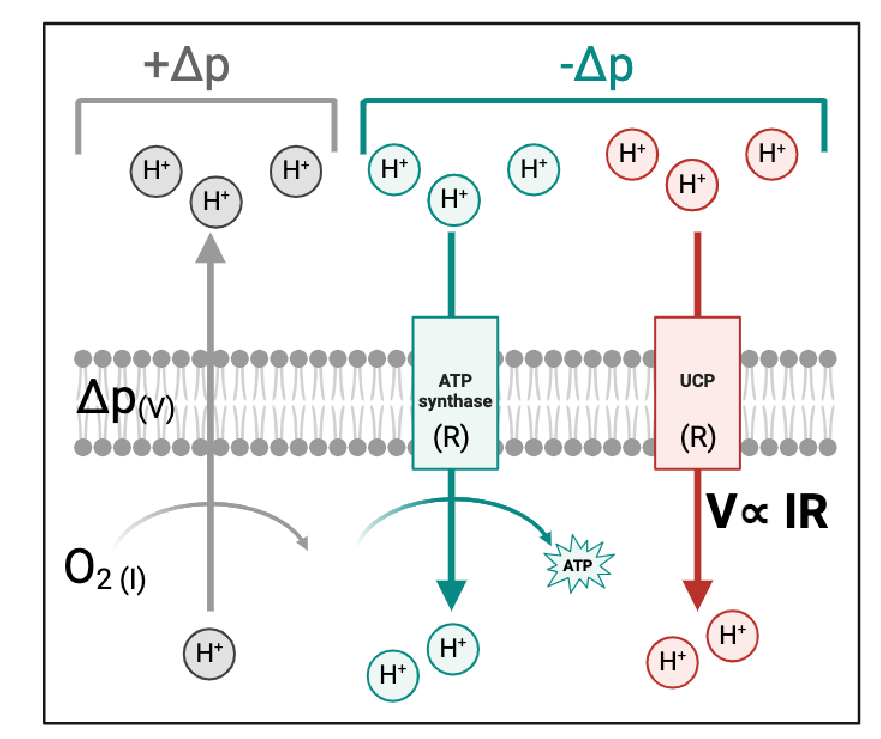
\includegraphics[width=\textwidth]{./main_plots/uncoupling_cartoon.png}        
    %     \end{subfigure}  
    %     \begin{subfigure}[t]{\textwidth}
    %         \caption{}
    %         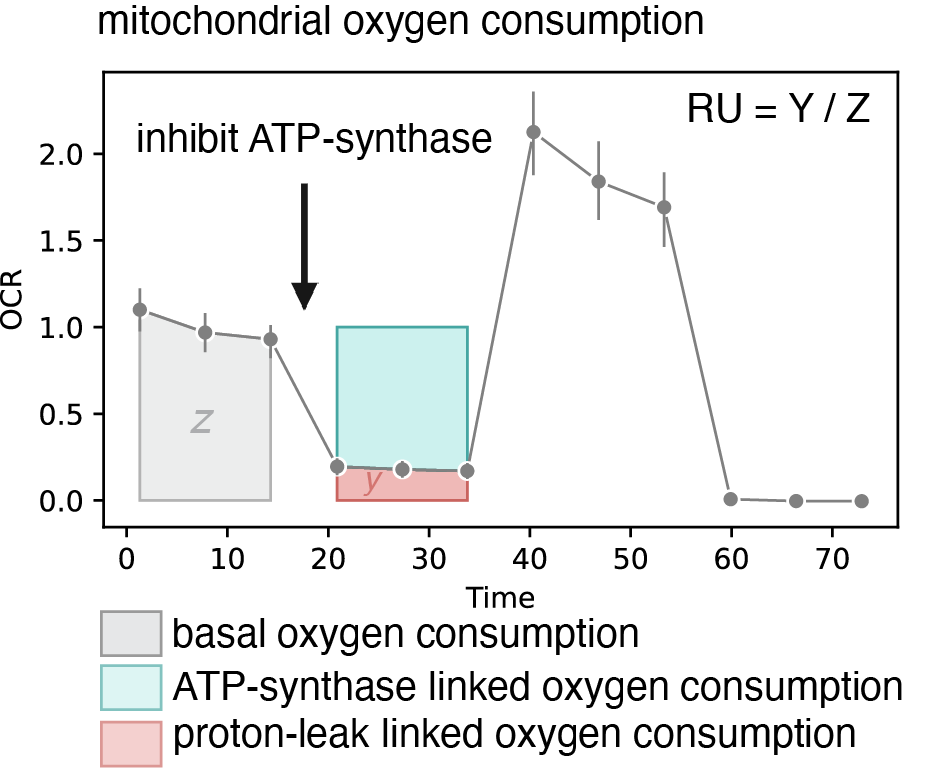
\includegraphics[width=\textwidth]{./main_plots/seahorse_cartoon.png}        
    %     \end{subfigure}      
    % \end{subfigure} 
    % \begin{subfigure}[t]{.15\textwidth}
    %     \caption{}
    %     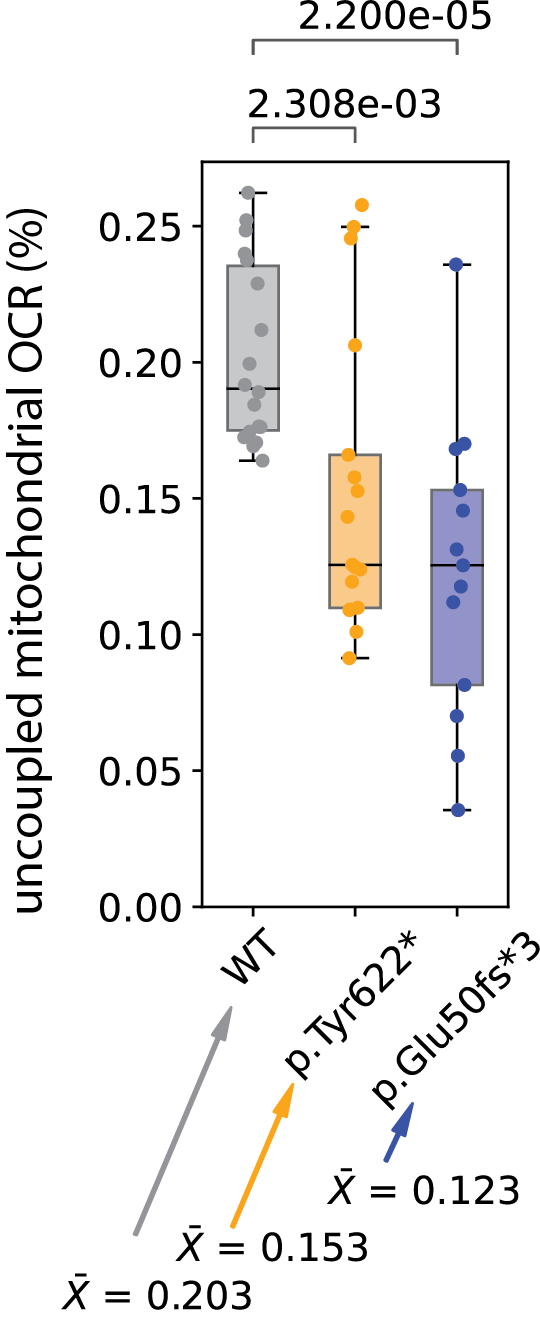
\includegraphics[width=\textwidth]{./main_plots/uncoupling.png}        
    % \end{subfigure}  
    % \begin{subfigure}[t]{.3\textwidth}
    %     \caption{}
    %     \includegraphics[width=\textwidth]{TMRM.png}        
    % \end{subfigure}  
    \caption{
        \textbf{ABCA7 LoF Impairs Regulation of Mitochondrial Uncoupling and Carbon Flux in Neurons.}\\[1ex]
        (A) Projection of WT and p.Glu50fs*3 metabolomes (per-sample z-scaled normalized peak areas; $N=6$ per genotype) onto the first two principal components from metabolite space. Fraction of explained variance shown along each axis. The dotted red line separating the two genotypes indicates the median PC1 value. 
        (B) Volcano plot indicating differentially regulated metabolites by log2-fold-change and log10(p-value), where log2(FC) > 0 indicates increased abundance in p.Glu50fs*3 vs. WT. Top up- and down-regulated metabolites are shown in red and blue, respectively (p-values by independent sample t-test). 
        (C) Abundance of carnitine species in WT vs. p.Glu50fs*3 iNs. 
        (D) Correlation of carnitine species abundance (normalized peak areas by LC-MS) and monoglyceride (MG) abundance (peak areas by LC-MS) from matched metabolomic-lipidomic samples. Grey points indicate WT iNs ($N=6$). Blue points indicate p.Glu50fs*3 iNs ($N=6$). The equation indicates the linear function fit. Grey error bar indicates 95\% confidence interval. 
        (E) Schematic indicating the relationship between oxygen consumption as a measure of proton current (I), which sustains the proton motive force ($\Delta p$; voltage (V)). Regulation of ATP synthase and uncoupling protein (UCP) activity modifies resistance (R) and depletes $\Delta p$. 
        (F) Schematic indicating how relative uncoupling is computed from oxygen consumption rate (OCR). Remaining oxygen consumption after pharmacological inhibition of ATP synthase gives the proportion of basal oxygen consumption attributed to proton leak. 
        (G) Relative uncoupling quantified by Seahorse oxygen consumption assay (see Methods) in 4-week-old WT vs. ABCA7 LoF iNs. P-values computed by independent sample t-test. $N$ wells = 18 (WT), 17 (p.Tyr622*), 13 (p.Glu50fs*3) across two independent differentiation batches and Seahorse experiments (see Figure~\ref{fig:snRNA_cohort}1E). 
        (H) Left: Quantification of neuronal HCS MitoHealth dye fluorescence intensity as a measure of mitochondrial membrane potential. P-values computed by linear mixed-effects model on per-NeuN+ volume averages, including well-of-origin as a random effect. $N=8$ (WT), 11 (p.Tyr622*), 9 wells (p.Glu50fs*3) (3000 cells per condition) from three independent differentiation batches (see Figure~\ref{fig:snRNA_cohort}1F). Individual data points indicate per-well averages of cell-level intensities. Right: Representative images per condition as mean-intensity projections of the entire image (NeuN+) and within NeuN+ volumes considered for quantification (MitoHealth, Hoechst). Representative images for the MitoHealth channel were processed with condition-wide percentile-based background subtraction and thresholding. Representative images of cell soma underwent per-image percentile-based background subtraction and thresholding, reflecting the segmentation methodology. For (C, G, H) boxes indicate per-condition dataset quartiles, and whiskers extend to the most extreme data points not considered outliers (i.e., within 1.5 times the interquartile range from the first or third quartile). 
    }
    \label{fig:main_mitochondrial}
\end{figure}